\chapter{Experimental Methods}
This chapter will cover the experimental methods used in the development of optomechanical systems, focusing on the generation of squeezed light and the techniques for optical locking and quadrature measurement. The methods are designed to enhance the sensitivity of measurements in quantum optics and optomechanics.
\minitoc
\newpage
\section{Optical Locking Techniques with PyRPL}
A central aspect of the experimental setups is the ability to stabilize various optical features. In this work, it is the case for the relative phase between two optical paths, keeping optical cavities on resonance, or fixing the detuning between a master and a slave laser. \newline

\noindent This section will cover the locking techniques used in this work, from basic Michelson-type locking to more advanced Pound-Drever-Hall techniques and phase-locked loops. The implementation of these techniques using the in-house library PyRPL is presented. 

\subsection{Proportion-Integral (PI) Controllers}
Proportional-Integral (PI) controllers are widely used in quantum optics experiments to stabilize critical parameters such as cavity length, laser frequency, and optical phase. To this end, one needs to extract an error signal \( \epsilon(t) \) that quantifies the deviation from a desired setpoint, such as a target temperature, phase difference or cavity resonance. It is typically expressed as the difference between a measured signal and its reference value:
\[
\epsilon(t) = s_{\text{meas}}(t) - s_{\text{ref}},
\]
where \( s_{\text{meas}}(t) \) denotes the physical quantity monitored in the experiment (e.g., reflected intensity or interferometric signal), and \( s_{\text{ref}} \) is the target value corresponding to the lock point.\newline

\noindent For effective feedback stabilization, the error signal must satisfy several essential criteria:
\begin{itemize}
    \item \textbf{High SNR:} Near the setpoint, \( \epsilon(t) \) should exhibit a high SNR to ensure robust locking and minimize the influence of technical and electronic noise.
    \item \textbf{Linearity and antisymmetry:} The error signal should be linear and antisymmetric in a neighborhood of the operating point. Small deviations from the setpoint should produce a proportional response in \( \epsilon(t) \), with opposite signs for deviations of opposite direction.
    \item \textbf{Monotonicity and uniqueness:} The slope \( \partial \epsilon / \partial x \), where \( x \) denotes the control parameter (e.g., cavity length or laser frequency), should be monotonic and unambiguous near the lock point to avoid multiple equilibrium points and ensure stable locking behavior.
    \item \textbf{Steep slope near the setpoint:} A steeper slope improves sensitivity to small deviations and enhances lock accuracy, although it must be balanced against potential noise amplification.
    \item \textbf{Bandwidth compatibility:} The spectral content of \( \epsilon(t) \) must be compatible with the bandwidth of the actuator and the dynamics of the system. For example, in the case of a piezoelectric transducer, which acts as a low-pass mechanical element, the error signal high-frequency components won't be compensated by the actuator.  
\end{itemize}

\noindent The PI controller computes the feedback signal \( u(t) \) from the error signal \( \epsilon(t) \) according to:
\begin{equation}
    u(t) = K_P \, \epsilon(t) + K_I \int_0^t \epsilon(\tau) d\tau
    \tag{III.1}
\end{equation}
where \( K_P \) and \( K_I \) are the proportional and integral gains, respectively. The proportional term \( K_P \, e(t) \) responds to the current error and primarily acts on mid-frequency deviations, enabling rapid corrections. The integral term \( K_I \int \epsilon(\tau) d\tau \) accumulates past errors and is most effective at low frequencies, helping to eliminate long-term drifts and steady-state offsets. \newline

\noindent In classical control theory, PID (Proportional-Integral-Derivative) controllers are designed to stabilize dynamic systems by combining three terms: a proportional term for immediate response, an integral term to eliminate steady-state error, and a derivative term that anticipates future error based on the rate of change. However, in practical experimental setups—particularly in quantum optics—PI control (Proportional-Integral) is typically sufficient and even preferable to full PID control. The derivative term, which acts predominantly at high frequencies, is generally unnecessary and can be counterproductive. This is because the feedback actuator is often a piezoelectric transducer, which exhibits non-zero capacitance. Combined with the finite output impedance of the control electronics, this forms a natural low-pass filter that significantly attenuates high-frequency components of the feedback signal. As a result, any derivative term—which primarily targets high-frequency correction—would be both ineffective due to this filtering and potentially harmful by injecting high-frequency noise into the loop. \newline 

\noindent Therefore, PI control offers a balanced and robust approach: the integral term suppresses low-frequency drifts (typically below a few Hz to tens of Hz), the proportional term corrects intermediate-frequency deviations (up to a few kHz), and high-frequency components (above the mechanical resonance or actuation bandwidth) are naturally filtered out and deliberately left uncorrected. This allows for stable feedback while preserving high-frequency signals—such as thermal noise or mechanical sidebands—which carry essential physical information for analysis and measurement.

\subsection{Temperature Locks}
A first example of a PI lock used in this work is the temperature lock, which is used to stabilize the temperature of non linear crystals embedded inside optical cavities. The error signal is derived from a temperature sensor, such as a thermistor, which measures the temperature of the crystal. The error signal is then fed into a PI controller, which adjusts the heating element, a peltier module in our case, to maintain the desired temperature setpoint. \newline

\noindent The temperature lock is crucial for maintaining the phase matching conditions in nonlinear optical processes (developped in the next section), such as second-harmonic generation or optical parametric oscillation, where the efficiency of frequency conversion depends sensitively on the crystal temperature. By stabilizing the temperature, we ensure that the nonlinear interactions remain optimal, leading to consistent and reproducible results in experiments involving squeezed light generation or other nonlinear optical phenomena. \newline



\subsection{Optical paths Locks}
Controlling the relative path length between two arms of an interferometer is a fundamental technique in quantum optics. The basic idea is to use the interference of light from two paths to lock the phase difference between them. Although not being the same experiental setups, Michelson interferometers, Mach-Zhender interferometers, and Local Oscillator stabilization error signals fall in the same category as they are derived from the same principle. Namely, the error signal is proportional to the sine of the phase difference between the two arms: 
\begin{align}
\epsilon(\Delta \phi) \propto  \sin(\Delta \phi) 
\end{align}
where $\Delta \phi = \phi_a - \phi_b$ is the phase difference between the two optical paths. Analogically, we would need to add an adjustable voltage offset, as to be able to tune the error signal to zero at the desired phase difference, before seeding this error signal to the PI block. Digitally, this is performed by adding a constant offset to the error signal, which can be adjusted to set the desired phase difference. \newline

\noindent In practice, this is implemented by mounting a mirror on which one of the arms is reflected, and then using a piezoelectric transducer to control the position of the mirror, hence modulating the relative phase between the two optical paths. The piezo is then feedback controlled through a PI loop, which adjusts the voltage applied to the piezo to set the error signal to 0. 
FIGURE 

\subsection{Side of Fringe Locks}

\subsection{Pound-Drever-Hall Locks}
Another key technique extensively used in this work is the \textit{Pound-Drever-Hall} (PDH) method, a high-sensitivity scheme for stabilizing either the cavity length to a fluctuating laser frequency, or vice versa. The method relies on imposing phase modulation sidebands on the laser field, typically using an electro-optic modulator (EOM), and using these sidebands as phase-stable references. Because they lie far outside the cavity linewidth (\( \Omega_{\text{mod}} \gg \kappa \)), the sidebands are reflected nearly unchanged: \( r(\omega_\ell \pm \Omega_{\text{mod}}) \approx 1 \). In contrast, the carrier field near resonance acquires a frequency-dependent phase shift upon reflection, captured by the complex cavity reflection coefficient \( r_c(\delta) \). The PDH error signal is obtained by detecting the reflected beam and demodulating the photocurrent at the modulation frequency, isolating the beat terms between carrier and sidebands. The resulting signal is proportional to the \textit{imaginary part} of \( r_c(\delta) \), which varies antisymmetrically with detuning and provides a zero-crossing error signal ideal for linear feedback. This imaginary component encodes the rapid phase dispersion near resonance that allows the system to discriminate the sign and magnitude of frequency deviations. In contrast, the real part of \( r_c(\delta) \), being symmetric around resonance, does not yield a usable error signal. \newline

\noindent The \textit{demodulation phase} plays a critical role in selecting the appropriate quadrature of the signal for feedback. Since the beat signal between the carrier and sidebands has both in-phase (cosine) and quadrature (sine) components, choosing the correct demodulation phase ensures that the extracted error signal aligns with the imaginary part of the reflection coefficient. A misaligned demodulation phase can lead to mixing of the symmetric (real) part into the error signal, thereby reducing sensitivity and introducing offset or distortion near the lock point. In practice, the demodulation phase is optimized empirically---either via a variable phase shifter in the electronic demodulation path or by adjusting the physical delay in the reference oscillator---to maximize the slope of the error signal at zero-crossing, corresponding to pure detection of the dispersive component.
\begin{figure}[htbp]
    \centering
    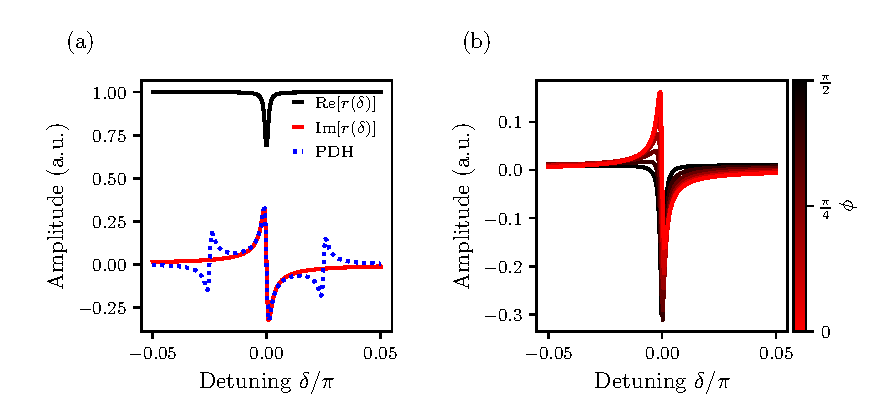
\includegraphics[width=\textwidth]{./chap3/fig/PDHplots.pdf}
    \caption{
        Schematic of the Pound-Drever-Hall (PDH) locking technique. 
        The laser passes through an electro-optic modulator (EOM) generating phase modulation sidebands. 
        The modulated beam is incident on the optical cavity, and the reflected light is detected by a photodiode (PD). 
        The photocurrent is demodulated at the modulation frequency to produce the PDH error signal, which is fed to a PI controller driving the cavity actuator (e.g., piezo). 
        Key components are labeled: EOM (electro-optic modulator), PD (photodiode), LO (local oscillator for demodulation), and PI (proportional-integral controller).
    }\label{fig:PDH_scheme}
\end{figure}

\noindent
The \textit{lock-in optical phase-sensitive error measurement} (LOPSEM) technique is a versatile method for extracting phase information from modulated optical signals. In the context of PDH locking, LOPSEM is used to demodulate the photodiode signal at the modulation frequency, isolating the dispersive error signal required for feedback. By employing a lock-in amplifier or digital demodulation, the technique enables precise selection of the signal quadrature, allowing for robust discrimination of phase shifts induced by cavity detuning. This approach enhances the sensitivity and stability of optical locks, making it an essential tool in quantum optics experiments where accurate phase control is critical.



\subsection{Offset frequency Locks}

coucou Marie 

\subsection{Coherent Sideband Locks}
\subsection{PyRPL Control Implementation}

\section{Optical Cavities and Squeezed Light Generation}
Maybe I need to add a section on the theory of squeezed light generation, but for now I will just focus on the experimental methods.
\subsection{Cavity Types and Alignement Procedures}


\subsection{Bowtie-type Optical Parametric Oscillator (OPO)}
\subsection{Phase Matching and Nonlinear Crystals}
\subsection{Filter Cavities for Squeezing Rotation}

\section{Quadrature Measurement Techniques}
\subsection{Direct Detection with Photodiodes}
\subsection{Balanced Homodyne Detection}
\subsection{Local Oscillator Design and Control}
\newpage
